\documentclass[12pt]{article}
\usepackage[utf8]{inputenc}

\usepackage{lmodern}

\usepackage{enumitem}
\usepackage[margin=2cm]{geometry}

\usepackage{amsmath, amsfonts, amssymb}
\usepackage{graphicx}
%\usepackage{subfigure}
\usepackage{tikz}
\usepackage{pgfplots}
\usepackage{multicol}

\usepackage{comment}
\usepackage{url}
\usepackage{calc}
\usepackage{subcaption}
\usepackage[indent=0pt]{parskip}
\usepackage{animate}

\usepackage{array}
\usepackage{blkarray,booktabs, bigstrut}
\usepackage{bigints}

\pgfplotsset{compat=1.16}

% MATH commands
\newcommand{\ga}{\left\langle}
\newcommand{\da}{\right\rangle}
\newcommand{\oa}{\left\lbrace}
\newcommand{\fa}{\right\rbrace}
\newcommand{\oc}{\left[}
\newcommand{\fc}{\right]}
\newcommand{\op}{\left(}
\newcommand{\fp}{\right)}

\newcommand{\bi}{\mathbf{i}}
\newcommand{\bj}{\mathbf{j}}
\newcommand{\bk}{\mathbf{k}}
\newcommand{\bF}{\mathbf{F}}

\newcommand{\mR}{\mathbb{R}}

\newcommand{\ra}{\rightarrow}
\newcommand{\Ra}{\Rightarrow}

\newcommand{\sech}{\mathrm{sech}\,}
\newcommand{\csch}{\mathrm{csch}\,}
\newcommand{\curl}{\mathrm{curl}\,}
\newcommand{\dive}{\mathrm{div}\,}

\newcommand{\ve}{\varepsilon}
\newcommand{\spc}{\vspace*{0.5cm}}

\DeclareMathOperator{\Ran}{Ran}
\DeclareMathOperator{\Dom}{Dom}

\newcommand{\exo}[1]{\noindent\textcolor{red}{\fbox{\textbf{Problem {#1}}}\hrulefill}\\}
\newcommand{\qu}[4]{\noindent\textcolor{#4}{\fbox{\textbf{Section {#1} | Problem {#2}}} \hrulefill{{\fbox{\textbf{{#3} Points}}}}\\}}

\newcommand{\semester}{Spring 2023}

\newcommand{\CVup}{%

\begin{tikzpicture}
\draw[black, <->, >=latex] (-0.33, 0.5) .. controls (-0.125, 0) and (0.125, 0) .. (0.33, 0.5);
\end{tikzpicture}}

\newcommand{\CVupInc}{%
\begin{tikzpicture}
\draw[black, ->, >=latex] (0,0) .. controls (0.2, 0) and (0.4, 0.2) .. (0.5, 0.5);
\end{tikzpicture}}

\newcommand{\CVupDec}{%
\begin{tikzpicture}[rotate=270]
\draw[black, ->, >=latex] (0,0) .. controls (0.2, 0) and (0.4, 0.2) .. (0.5, 0.5);
\end{tikzpicture}}

\newcommand{\CVdown}{%
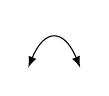
\begin{tikzpicture}
\draw[black, <->, >=latex] (-0.33, -0.5) .. controls (-0.125, 0) and (0.125, 0) .. (0.33, -0.5);
\end{tikzpicture}}

\newcommand{\CVdownInc}{%
\begin{tikzpicture}
\draw[black, ->, >=latex] (-0.5, -0.5) .. controls (-0.5, -0.3) and (-0.5, -0.1) .. (0,0);
\end{tikzpicture}}

\newcommand{\CVdownDec}{%
\begin{tikzpicture}[rotate=-90]
\draw[black, ->, >=latex] (-0.5, -0.5) .. controls (-0.5, -0.3) and (-0.5, -0.1) .. (0,0);
\end{tikzpicture}}

\begin{document}
	\noindent \hrulefill \\
	MATH-241 \hfill Pierre-Olivier Paris{\'e}\\
	Solutions Section 2-3 \hfill \semester \\\vspace*{-1cm}
	
	\noindent\hrulefill
	
	\spc
	
	\exo{2}
	\\
	Don't get confused, $\pi$ is a constant (it does not depend on $x$). So $\pi^2$ is a constant. Then $f'(x) = 0$.
	
	\spc
	
	\exo{4}
	\\
	Using the fact that the derivative of a sum is the sum of the derivatives and the power rule, we have
		\begin{align*}
		g'(x) = \frac{dg}{dx} &= \frac{d}{dx} \op \frac{7}{4} x^2 \fp - 3 \frac{d}{dx} (x) + \frac{d}{dx}(12) \\
		&= (7/4) 2 x - 3 (1) + 0 \\
		&= (7/2)x - 3 .
		\end{align*}
	Therefore, $g'(x) = (7/2)x - 3$.
	
	\spc
	
	\exo{18}
	\\
	Using the quotient rule, we obtain
		\begin{align*}
		y' = \frac{(\sqrt{x} + x)' x^2 - (\sqrt{x} + x) (x^2)'}{x^4} .
		\end{align*}
	We have, from the power rule,
		\begin{align*}
		(\sqrt{x} + x)' = 1/2\sqrt{x} + 1 \quad \text{ and } \quad (x^2)' = 2x
		\end{align*}
	and so replacing that in $y'$, we obtain
		\begin{align*}
		y' = \frac{(1/2\sqrt{x} + 1) x^2 - (\sqrt{x} + x) 2x}{x^4} = \frac{x^{3/2}/2 + x^2 - 2x^{3/2} - 2x^2}{x^4} = \frac{-3x^{3/2}/2 - x^2}{x^4} .
		\end{align*}
	Finally, we get $y' = -3x^{-5/2}/2 - x^{-2}$.
	
	There is another approach. By letting $x \neq 0$, we can rewrite the expression as
		\begin{align*}
		y = x^{-3/2} + x^{-1}
		\end{align*}
	and by the sum and quotient rules, we obtain
		\begin{align*}
		y' = -3 x^{-5/2}/2 - x^{-2} .
		\end{align*}
	
	\newpage
	
	\exo{26}
	\\
	Using the product rule, we have
		\begin{align*}
		B'(u) = (2u^2 - 4u - 1) \frac{d}{du} (u^3 + 1) + (u^3 + 1) \frac{d}{du} (2u^2 - 4u - 1) .
		\end{align*}
	Then, using the sum rule and the power rule for derivatives, we get
		\begin{align*}
		\frac{d}{du} (u^3 + 1) = 3u^2
		\end{align*}
	and
		\begin{align*}
		 \frac{d}{du} (2u^2 - 4u - 1) = 4u - 4 .
		\end{align*}
	Plugging in back in $B'(u)$, we get
		\begin{align*}
		B'(u) = (2u^2 - 4u - 1)3u^2 + (u^3 + 1)(4u - 4) &= 6u^4 - 12u^3 - 3u^2 + 4u^4 - 4u^3 + 4u - 4 \\
		&= 10u^4 - 16u^3 - 3u^2 + 4u - 4 .
		\end{align*}
	Therefore, $B'(u) = 10u^4 - 16u^3 - 3u^2 + 4u - 4 $.
	
	\spc
	
	\exo{30}
	\\
	Using the quotient rule, we get
		\begin{align*}
		h'(t) &= \frac{(6t - 1)\frac{d}{dt} (6t + 1) - (6t + 1) \frac{d}{dt}(6t - 1)}{(6t - 1)^2} \\
		&= \frac{(6t - 1) 6 - (6t + 1) 6}{(6t - 1)^2} \\
		&= - \frac{12}{(6t - 1)^2} .
		\end{align*}
	
	\spc
	
	\exo{54}
	\begin{enumerate}[label=\textbf{(\alph*)}]
	\item We first find the derivative. We get
		\begin{align*}
		y' = \frac{1 + x^2 - 2x^2}{1 + x^2} = \frac{1 - x^2}{(1 + x^2)^2} .
		\end{align*}
	The equation of the tangent line is given by the equation $y - 0.3 = y'(3) (x - 3)$. So, pugging in the numbers, with $y' = -8/100 = -2/25$, we obtain
		\begin{align*}
		y - 0.3 = (-2/25)(x - 3) \Rightarrow y = (-0.08)x + 0.54 .
		\end{align*}
	\item Using Desmos, we get the following picture.
		\begin{figure}[h]
		\centering
		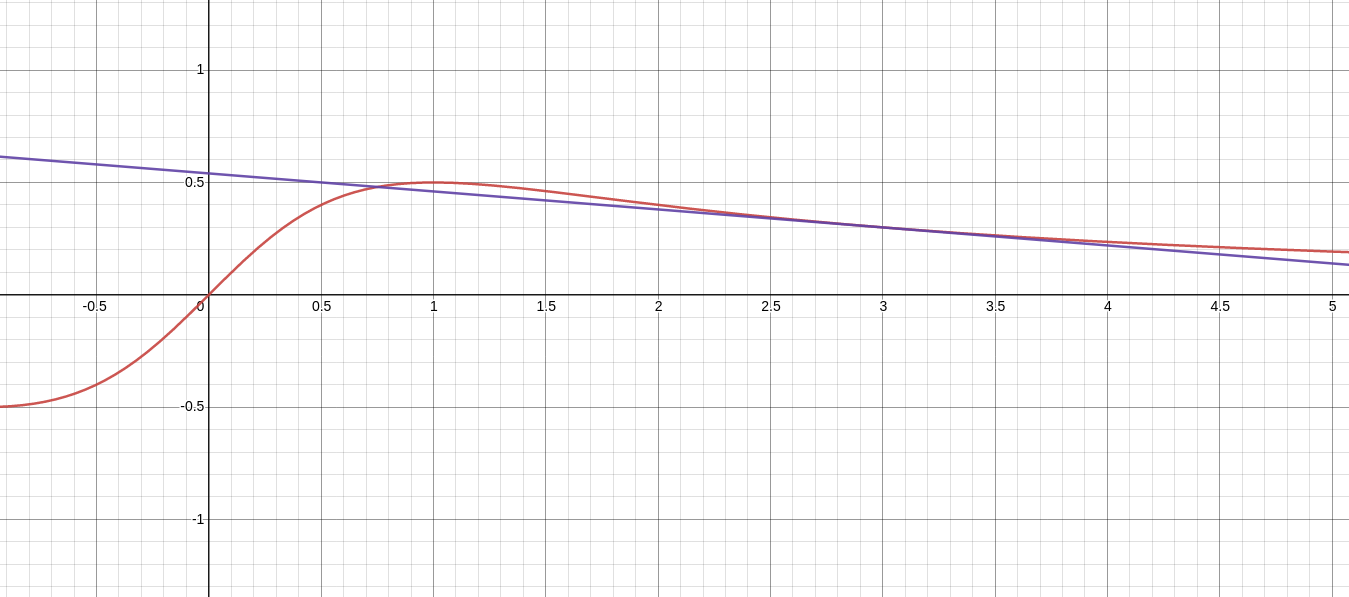
\includegraphics[scale=0.32]{problem54b.png}
		\end{figure}
	\end{enumerate}
	
	\spc
	
	\exo{58}
	\\
	The equation of the tangent line at $(4, 0.4)$ is
		\begin{align*}
		y - 0.4 = f'(0.4) (x - 4) .
		\end{align*}
	We have $f(x) = \sqrt{x}/(x + 1)$. Using the quotient rule, we get
		\begin{align*}
		f'(x) = \frac{\frac{x + 1}{2\sqrt{x}} - \sqrt{x}}{(x + 1)^2} = \frac{1 - x}{2\sqrt{x}(x + 1)^2} .
		\end{align*}
	Therefore, we have $f'(4) = -0.03$. Plugging this into the equation of the tangent line and after simplifying, we get
		\begin{align*}
		y = 0.52 - 0.03x .
		\end{align*}
		
	\spc
	
	\exo{66}
	\\
	Using the power rule for derivatives, we see that
		\begin{align*}
		S'(A) = (0.882)(0.842)A^{-0.158} = (0.742644)A^{-0.158}.
		\end{align*}
	Using the formula for $S'(A)$, we find that
		\begin{align*}
		S'(100) = (0.882)(0.842)(100)^{-0.158} \approx 0.35874 \text{ trees}/\text{m}^2
		\end{align*}
	where $\text{m}^2$ means square meters.
	
	\newpage
	
	\exo{72}
	\\
	Since the function $f(x) = x$ is not zero at $x = 2$, we can use the quotient rule. We obtain
		\begin{align*}
		\frac{d}{dx} \Big( \frac{h(x)}{x} \Big) = \frac{h'(x) x - h(x)}{x^2} 
		\end{align*}
	and then, at $x = 2$, we get
		\begin{align*}
		\frac{d}{dx} \Big( \frac{h(x)}{x} \Big) \Big|_{x = 2} = \frac{h'(2) \times 2 - h(2)}{4} = \frac{(-3) \times 2 - 4}{4} = -5/2 .
		\end{align*}
	
	
\end{document}